\section{Réalisation}

\subsection{Partie 1 -- Registre à décalage 4 bits}

Le registre est composé de 4 bascules D partageant la même horloge \texttt{clock\_i} et le même reset asynchrone \texttt{reset\_i}. Devant chaque bascule, un multiplexeur commandé par \texttt{en\_sh\_i} sélectionne la donnée à mémoriser : lorsque \texttt{en\_sh\_i} vaut 1, la première bascule reçoit l'entrée série \texttt{ser\_r\_i} et chacune des suivantes la sortie de la bascule précédente. Les sorties des bascules sont regroupées sur le bus \texttt{reg\_o}, la première bascule correspondant au bit de poids fort (bit 3), ce qui réalise un décalage vers la droite.

\begin{schema}
	\centering
	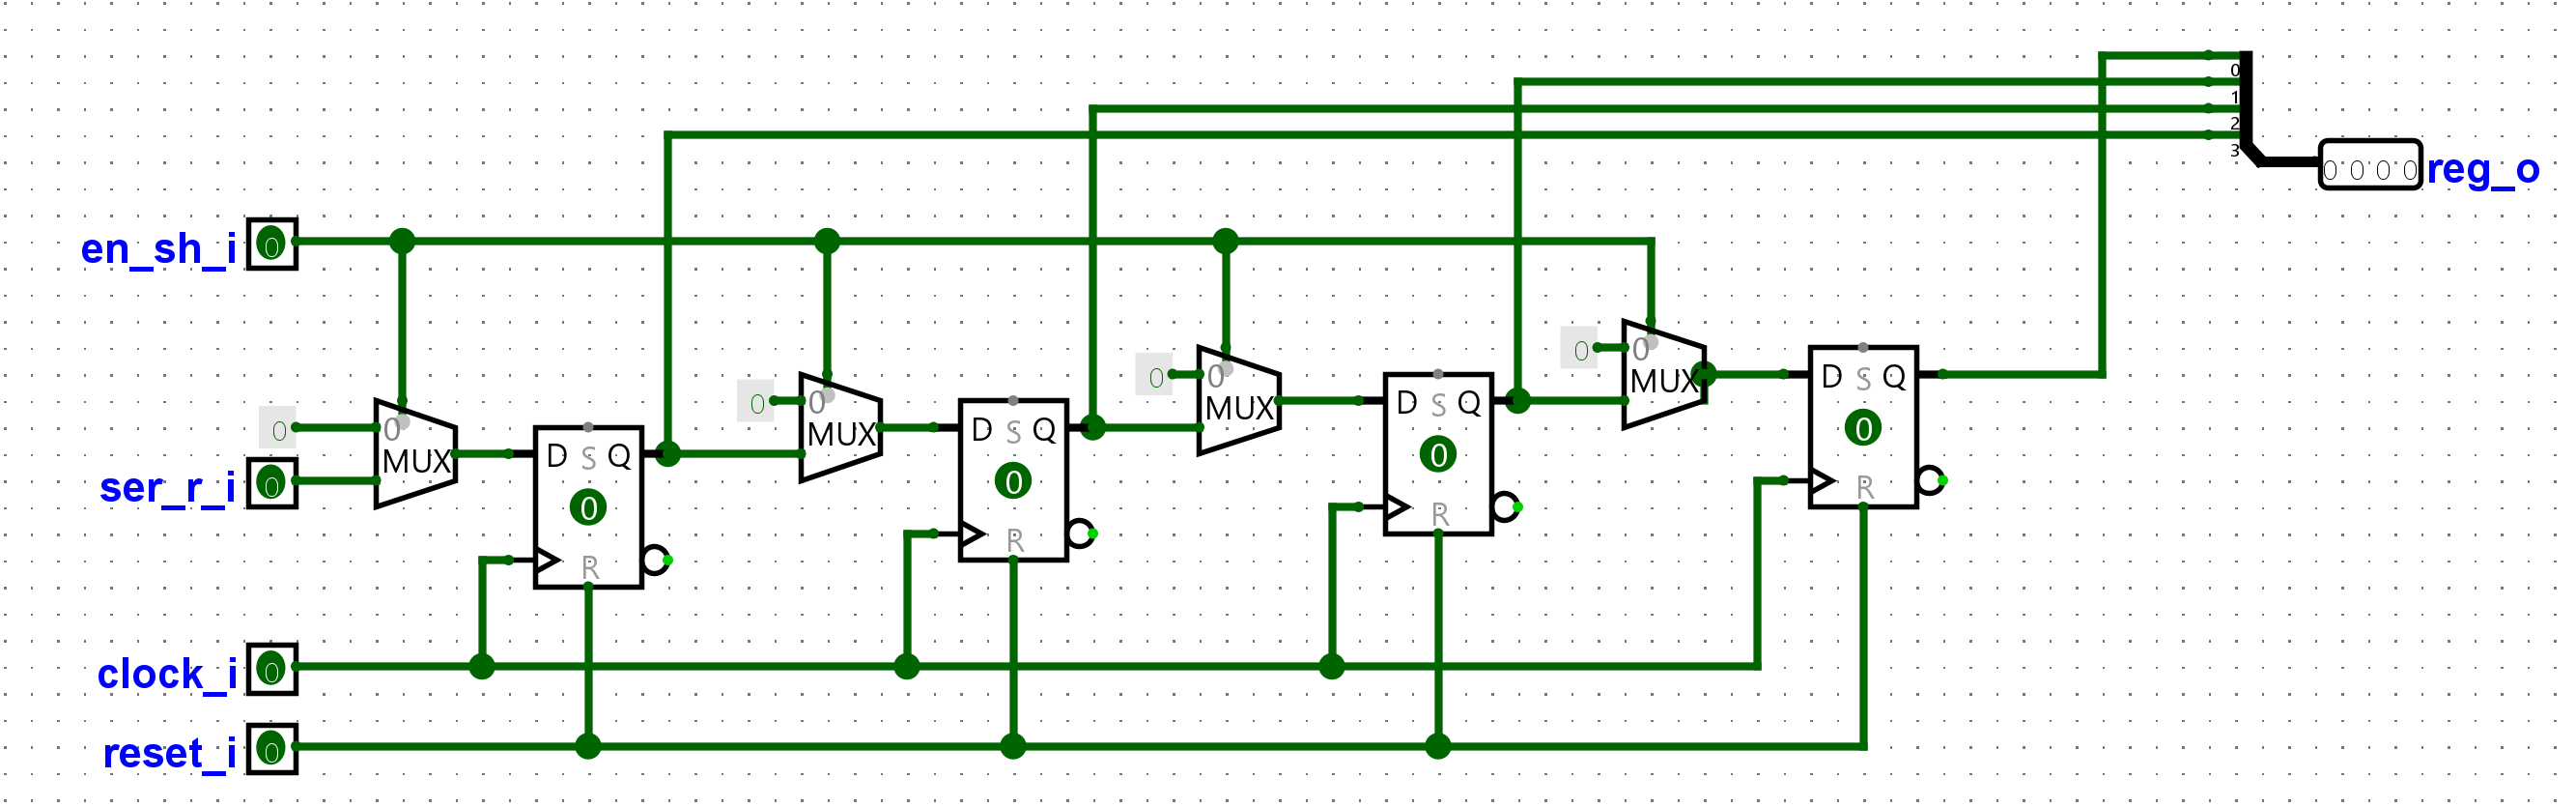
\includegraphics[width=\textwidth]{./images/schema-partie1-logisim.png}
	\caption{Logisim : registre à décalage 4 bits}
	\label{fig:schema_p1}
\end{schema}

\subsection{Partie 2 -- Registre à décalage 8 bits}

% \begin{schema}
% 	\centering
% 	\includegraphics[width=\textwidth]{./images/srg8_ld_sh.png}
% 	\caption{Logisim : registre à décalage 8 bits}
% 	\label{fig:schema_p2}
% \end{schema}

\subsection{Partie 3 -- Chenillard}

% \begin{schema}
% 	\centering
% 	\includegraphics[width=\textwidth]{./images/chenillard.png}
% 	\caption{Logisim : chenillard}
% 	\label{fig:schema_p3}
% \end{schema}
